%%% Local Variables: 
%%% mode: latex
%%% TeX-master: t
%%% End:

\documentclass[a4paper, 10pt]{article}

\usepackage[utf8]{inputenc}
\usepackage{hyperref}
\usepackage{enumerate}
\usepackage{multirow}
\usepackage{wrapfig}

\usepackage{fancyvrb}
\DefineVerbatimEnvironment{code}{Verbatim}{fontsize=\small}
\DefineVerbatimEnvironment{example}{Verbatim}{fontsize=\small}

\usepackage{graphicx}
% \usepackage[margin=2cm]{geometry}
\usepackage[backend=bibtex]{biblatex}
\addbibresource{references.bib}

\title{Software Reengineering\\
       Assignment 1}
\author{Joey Ezechi\"{e}ls (1338994) \and Volker Lanting (1513273)}

% % Implement x.yy numbering scheme for subsections
% % where yy is *always* a 2-digit number
% \makeatletter
% \renewcommand\thesubsection{\thesection.\two@digits{\arabic{subsection}}}
% \makeatother

\begin{document}
\maketitle % Doesn't count towards the total number of pages
\pagenumbering{roman}

\newpage
\tableofcontents % Doesn't count towards the total number of pages

% \newpage
% \section{Introduction}
% \label{sec:introduction}

\newpage
\pagenumbering{arabic}
\section{Initial Questions}
\label{sec:initial_question}
In reverse-engineering the JMonkeyEngine, there are some initial
questions that need answering in order to gain a clearer picture
of what the architecture and code look like.

% For each of these pieces of code, reasons why they violate the
% principles *must* be provided. We must use figures and/or metrics to
% underline our reasoning.

% Simple shortcomings in the source code don't count, such as code
% clones of 1-2 lines, naming, or missing comments.

\subsection{Main features of the program}
\label{sec:main_features}
% What are the main features of the program?

jMonkeyEngine can be used to create games. To this end it offers a
number of features, among which we consider the following ones the
most important:
\begin{itemize}
	\item Creating Applications 
	(\verb|com.jme3.app|, \verb|com.jme3.system|)
	\item Managing Assets of these applications (\verb|com.jme3.asset|)
	The main assets are scenes, 
	located in the \verb|com.jme3.scene| package.
	% \begin{itemize}
	% 	\item Animations (\verb|com.jme3.animation|)
	% 	\item Meshes (\verb|com.jme3.scene|)
	% 	\item Textures (\verb|com.jme3.texture|)
	% 	\item 2D Pictures (\verb|com.jme3.ui|)
	% 	\item Scenes
	% 	(referred to as Spatial in the code \verb|com.jme3.scene|)
	% 	\item Materials (\verb|com.jme3.material|)
	% 	\item Shaders (\verb|com.jme3.shader|)
	% \end{itemize}
	
	\item Real time Rendering (\verb|com.jme3.renderer|)
	% \item Creating Particle effects (\verb|com.jme3.effect|)
	% \item Creating post processing effects (\verb|com.jme3.post|)
	\item Collision detection (\verb|com.jme3.collision|, \verb|com.jme3.bounding|)
	% \item Cinematic events and motion paths (\verb|com.jme3.cinematic|)
	% \item Exporting assets (\verb|com.jme3.export|)
	% \item Support for fonts (\verb|com.jme3.font|, \verb|com.jme3.renderer|)
	% \item Dealing with user input (\verb|com.jme3.input|)
	% \item Lighting of a scene (\verb|com.jme3.light|, \verb|com.jme3.shadow|)
	\item Shaders (\verb|com.jme3.shader|)
\end{itemize}


\subsection{Important source code entities}
\label{sec:important_src_entities}
% Which are the important source code entities?

\begin{tabular}{| c | c |}
  \hline
  \textbf{Feature}                  & \textbf{Important source entities} \\
  \hline
  \hline
  Managing assets                   & AssetManager, ImplHandler, \\
				    & Node, Mesh, Geometry, Spatial \\
  \hline
  Creating applications             & SimpleApplication \\
  \hline
  Managing/configuring applications & AppSettings, JmeSystem, \\
                                    & JmeSystemDelegate, \\
                                    & AbstractAppState, AppStateManager \\
  \hline
  Real time rendering               & RenderManager, Camera,  \\
                                    & ViewPort, RenderQueue \\
  \hline
  Shaders                           & Shader, Uniform, \\
                                    & UniformBindingManager \\
  \hline
  Collision Detection		    & CollisionResults, BoundingVolume\\
  \hline
\end{tabular}
\newline
\newline
The actual Renderer is located in the lwjgl subsystem 
and not part of the core subsystem. 
Therefore we will skip them for this project.
 
% Volker

\subsection{Quality, Design and Implementation:\\First impressions}
\label{sec:first_impressions}
% What is your first impression of the quality of the design and
% implementation (also think of documentation, tests, etc.)?

% Joey

% Notes:
% - package structure is good
% - The code itself uses a lot of interfaces but also
%   shows signs of organic growth.
% - There is a tradeof between speed and design,
%   epecially in the com.jme3.math package

Our first impressions are that generally the package structure is
well-defined and the code itself uses a lot of interfaces, which
generally is a good sign (though of course not a conclusive indicator
of good design).

However there are also some odd design decisions (e.g. an inner enum in a
class that is referenced from a class in another package) design
violations (perhaps due to organic growth of the code base), and the
code base also shows signs that a tradeoff between execution speed and
design has been made, particularly in the \verb|com.jme3.math| package.

Generally the documentation seems fairly good and up to date
(e.g. there is a slide show on the website explaining how Scene Graphs
work in JME3). However in some parts of the code itself there seems to
be lack of comments, which would be helpful especially in the more
obscure parts of the code base.

Counting in absolute numbers, there is a fairly large set of tests.
However it interesting and somewhat disappointing that for the
entities we consider major there are almost no tests. For example,
the \verb|com.jme3test.math| and \verb|com.jme3test.scene| packages
contain only \textbf{1} and \textbf{2} tests, respectively.
Next to that it is quite surprising that the test packages are
different from the src packages (i.e. \verb|com.jme3test.math| is used
for tests rather than \verb|com.jme3.math|). While it is possible that
there are some considerations we don't know about, we consider it a
rather dumb decision as it makes testing package-private classes quite
a bit more difficult.


\subsection{Reengineering feasibility}
\label{sec:reengineering_feasibility}
% Do you think a reengineering is feasible?
Reengineering is feasible, as the current design and quality really isn't bad.
Also, since we don't have a specific goal for our reengineering 
(like making it easier to add a specific feature).


% Volker

\subsection{Exceptional entities}
\label{sec:exceptional_entities}
% What are the exceptional packages, classes and methods?

\begin{tabular}{|c|c|}
\hline
\multicolumn{2}{|c|}{\textit{Complexity per class}}\\
\hline
\textbf{Package} & \textbf{Classes}\\
\hline
\verb|com.jme3.math|			& FastMath, Quaternation, Matrices, Vectors\\
\hline
\verb|com.jme3.bounding|		& BoundingBox, BoundingSphere\\
\hline
\verb|com.jme3.scene|			& Node, Mesh, Geometry, Spatial\\
\hline
\verb|com.jme3.renderer|		& RenderManager, Caps\\
\hline
\verb|com.jme3.material|		& Material, MatParam\\
\hline
\verb|com.jme3.collision|		& SweepSphere\\
\hline

\hline
\multicolumn{2}{|c|}{\textit{Lack of cohesion (LCOM4)}}\\
\hline
\textbf{Package} & \textbf{Classes}\\
\hline
\verb|com.jme3.system|		& AppSettings, JmeSystemDelegate\\
\hline
\verb|com.jme3.math|		& Quaternation, ColorRGBA\\
\hline
\verb|com.jme3.scene|		& Node, SimpleBatchNode, Spatial\\
\hline
\verb|com.jme3.shader|		& Shader\\
\hline
\verb|com.jme3.asset|		& AssetKey, ImplHandler\\
\hline

\hline
\multicolumn{2}{|c|}{\textit{Too much responsibility (Afferent Coupling)}}\\
\hline
\textbf{Package} & \textbf{Classes}\\
\hline
\verb|com.jme3.math|		& Vector3f, FastMath, Quaternation,\\
                                & ColorRGBA, Matrix4f, Matrix3f\\
\hline
\verb|com.jme3.scene|		& Spatial, Mesh, VertexBuffer,\\
				& Geometry, Node\\
\hline
\verb|com.jme3.renderer|	& Camera, Viewport\\
				& Renderer, RenderManager\\
\hline
\verb|com.jme3.asset|		& AssetKey, AssetManager\\
\hline

\hline
\multicolumn{2}{|c|}{\textit{Instability (Efferent/Afferent coupling ratio)}}\\
\hline
\textbf{Package} & \textbf{Classes}\\
\hline
\verb|com.jme3.asset|		& DesktopAssetManager\\
\hline
\verb|com.jme3.scene|		& BatchNode\\
\hline
\verb|com.jme3.app|	        & SimpleApplication\\
\hline
\verb|com.jme3.collision|	& BIHTree, BIHNode\\
\hline
\verb|com.jme3.shader|		& Uniform, UniformBindingManager\\
\hline
\verb|com.jme3.bounding|	& BoundingBox, BoundingSphere\\
\hline
\end{tabular}\\\\

The \verb|com.jme3.math| package has quite some duplicate 
code blocks. Exceptional classes are LineSegment and Matrix4f.

\begin{tabular}{|c|c|c|}
\hline
\multicolumn{3}{|c|}{\bfseries Complex methods (CC)}\\
\hline
\textbf{Package}&\textbf{Class}&\textbf{Method}\\
\hline
\verb|com.jme3.math|	        & LineSegment	        & distanceSquared\\
\hline
			        & Matrix4f	        & get\\
\hline
			        &			& set\\
\hline
			        &			& equals\\
\hline
                                &			& equalIdentity\\
\hline
\verb|com.jme3.scene|	        & BatchNode	        & mergeGeometries\\
\hline
			        & Mesh		        & setInterleaved\\
\hline
\verb|com.jme3.scene.shape|	& Cylinder	        & updateGeometry\\
\hline
\verb|com.jme3.shader|	        & Uniform	        & setValue\\
\hline
				& UniformBindingManager	& updateUniformBindings\\
\hline
\verb|com.jme3.asset|	        & BlenderKey	        & equals\\
\hline
\verb|com.jme3.material|	& RenderState	        & contentHashCode\\
\hline
				& Material	        & read\\
\hline
				& MatParam	        & getValueAsString\\
\hline
\end{tabular}
% Volker (sonar):
% - packages
% - Search for methods ans classes that smell

% Joey (inCode):
% - god classes and general class & interface stuff
% - brain methods & feature envy

Also, a number of \textbf{God classes}, %\textbf{Brain methods} and
\textbf{Data classes} and a number of \textbf{Feature envy} and
\textbf{Code duplication} occurrences have been found
The 5 most egregious of each of these are:

\begin{tabular}{| l || c |}
  \hline
  % \textbf{Brain methods}    &  (),  () \\
  %                           &  (), \\
  %                           &  (),  () \\
  % \hline
  \textbf{Data classes}     & TempVars (50.5), RenderContext (19.25), \\
                            & Environment (14.25), \\
                            & TouchEvent (8.55), StringBlock (8.33) \\
  \hline
  \textbf{God classes}      & Material (81.03), Camera (35.37), \\
                            & RenderManager (33.99), \\
                            & BatchNode (24.96), BufferUtils (23.62) \\
  \hline
  \textbf{Feature Envy}     & BoundingBox.intersects (22), BIHTree.createBox (20) \\
                            & Ray.intersects (19), Camera.lookAt (15), \\
                            & TangentBinormalGenerator.linkVertices (14) \\
  \hline
  \textbf{Code Duplication} & LineSegment.distanceSquared (9.1), Matrix4f.get (7.4) \\
                            & Matrix3f.get (7.4), Texture3D.setWrap (6.9), \\
                            & TextureCubeMap.setWrap (6.9) \\
  \hline
\end{tabular}

% The numbers in braces represent the 

\subsection{Inheritance structure}
\label{sec:inheritance_structure}
% What does the inheritance structure look like?
Below are the most important parent classes that we found,
along with a short description on where they are implemented or inherited.

\begin{tabular}{|c|c|c|}
\hline
\textbf{Package}&\textbf{Entity}&\textbf{Subtyped in}\\
\hline
\verb|com.jme3.app.state |&
	AbstractAppState&
		states in \verb|com.jme3.app|\\

	% why are the implementations of this in the app package?
\hline
\verb|com.jme3.asset|&
	AssetKey&
	keys in \verb|asset|, \verb|shader|, \verb|scene|, \verb|audio|\\
\hline&
	AssetProcessor&
	processors in \verb|asset|, \verb|material|, \verb|texture|\\
\hline&
	CloneableSmartAsset&
	Material in \verb|material|,\\&& 
	Spatial in \verb|scene|\\&&
	Texture in \verb|texture|\\
\hline&
	AssetLoader&
	loaders in\\&&
	\verb|asset|, \verb|material|, \verb|texture|,\\&&
	\verb|scene|, \verb|audio|, \verb|font|, \\&&
	\verb|cursoris|, \verb|shader|, \verb|export|\\
\hline&
	AssetLocator&
	locators in plugins\\
\hline
\verb|com.jme3.collision|&
	Collidable&
	AbstractTriangle, Ray in \verb|math|,\\&&
	Spatial in \verb|scene|,\\&&
	BoundingVolume in \verb|bounding|,\\&&
	SweepSphere in \verb|collision|\\

\hline
\verb|com.jme3.scene|&
	Spatial&
	inherited by Node and\\&&
	Geometry from \verb|scene|,\\&&
	which are in turn inherited\\&&
	throughout the system\\
\hline&
	Mesh&
	used in all kinds of \\&&
	shapes in \verb|scene.shape|,\\&&
	\verb|scene.debug| and \verb|effect|\\
\hline
\verb|com.jme3.scene.control|&
	Control&
	implemented by AbstractControl \\&&
	in \verb|scene.control|,\\&&
	which is in turn extended \\&&
	in all kinds of Controls\\&&
	throughout the system\\
\hline
\end{tabular}


% Volker (& Joey)

\subsection{Scene composition: Basic elements}
\label{sec:scene_composition}
% What are the basic elements to compose a scene?
Scenes are represented as a scene graph.
This graph exists of Spatials, which represent (collections of) objects in space. 

There are two types of Spatials: Node and Geometry.
Nodes group other Spatials (their children) together, 
so all these children can be placed and moved relative to their parent.
A Geometry node represents an actual visible object in the scene.
It can not have children, but does have a Mesh (its shape in space) 
and a Material (determining its appearance).
% Volker

\subsection{Scene rendering}
\label{sec:scene_rendering}
% How is a scene rendered?

% Joey

\subsection{Collision detection}
\label{sec:collision_detection}
% How are collisions detected?

% in the com.jme3.bounding package for collision detection
% Bounding boxes are being made, check the code and the site
% for details

\newpage
\section{Problem detection}
\label{sec:problem_detection}

By utilising a number of tools available to us (see section
\ref{sec:used_tools} for details) and knowledge gained from this
course we have identified a number of shortcomings in both the design
and implementation of JMonkeyEngine. In searching for these
shortcomings we have kept in mind the  S.O.L.I.D. design principles,
though we have also considered the ADP and DRY principles.

% These questions must be answered:
% - What the exact problem is
% - Where the problem is
% - Why it is a problem

\subsection{Single Responsibility violation}
\label{sec:srp_violation}
% 2 examples of an Single Responsibility Principle violation
\subsubsection{JmeSystem}
JmeSystem seems to have too much responsibilities.
The lack of comments makes it hard to say anything about what 
the intended responsibility is, but it seems to be:
Manage permissions related to IO 
(isLowPermissions, getStorageFolder),
do image IO (writeImageFile),
manage system dependent data (getPlatform),
manage screen dialogs 
(setSoftTextDialogInput, showErrorDialog) and
serve as a factory for system related managing classes 
(newAssetManager, newAudioRenderer, createImageRaster).

There is clearly too much responsibility here, 
which is indicated by Sonar's LCOM4 metric.
This metric groups methods based on common attributes.
If there are two or more disjoint groups, 
there is a lack of cohesion between the methods of a class.
Usually, this is an indicator that there are two or more 
responsibilities for the class.

The LCOM4 method is easy to fool, as
abstract methods and loggers shared in methods can throw off
the LCOM4 measure.
The JmeSystem takes all its functionality 
from the abstract JmeSystemDelegate, 
which has an LCOM4 of 2,
and its subtype JmeDesktopSystem also has an LCOM4 of 2.

Inspection of some of the afferent couplings of JmeSystem 
leads to the following usage table, 
illustrating how breaking up the class will result in 
less coupling.

\begin{tabular}{|c|c|}
\hline
\textbf{Part}&\textbf{Usage}\\\hline
factory	& AwtPanelsContext\\\hline
		& Application\\\hline
		& ShaderCheck\\\hline
		& ImageRaster\\\hline
dialog	& InputSystemJme\\\hline
		& Application\\\hline
		& SimpleApplication\\\hline
permissions	& ClasspathLocator\\\hline
		& AppletHarness\\\hline
		& LwjglAbstractDisplay\\\hline
image IO	& ScreenshotAppState\\\hline
storage folder	& SaveGame\\\hline
		& ScreenshotAppState\\\hline
platform	& LwjglCanvas\\\hline
\end{tabular}

\subsubsection{Material}
Material is quite an exceptional entity,
with an efferent coupling of 42,
697 lines of code,
using 77 accessors or attributes of 24 unrelated classes,
having a complexity of 193 according to Sonar's check, and
triggering all four lack of cohesion of methods indicators of Eclipse Metrics.

\begin{figure}[htb!]
\centering
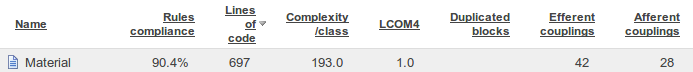
\includegraphics[width=\textwidth]{figures/material-sonar.png}
\vspace{-20pt}
\caption{some Sonar metrics for Material}
\label{fig:material-sonar}
\end{figure}
\vspace{-20pt}
\begin{figure}[htb!]
\centering
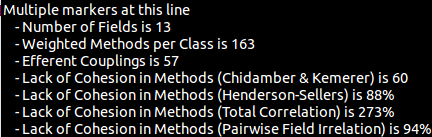
\includegraphics[width=70mm]{figures/material-metrics.png}
\vspace{-10pt}
\caption{some Eclipse Metrics results for Material}
\label{fig:material-metrics}
\end{figure}

It has gotten so big, complex and coupled that it is hard to 
figure out what it is doing, and even harder to believe
it is a single responsibility.
According to the javadoc comments, 
it has the following responsibility:
Material describes the rendering style for a given Geometry.
However, a Material is not specific for a given Geometry.
Nor is it purely a collection of parameters to configure
the style of rendering.
We think the real responsibilities of Material are:
describe a rendering style 
(MatParam, RenderState, Technique, transparent, receiveShadows),
and apply it to a Geometry and render it
(updateLightListUniforms, preload, render).

\subsection{Open-Closed Principle / Liskov Substitution Principle violation}
\label{sec:lsp_violation} % TODO if we choose OCP instead this should
                          % be changed to sec:ocp_violation
% one example of an Open/Closed Principle violation or 
% a Liskov substitution Principle violation

The enum \verb|com.jme3.shader.VarType| and the class
\verb|com.jme3.material.MatParam| violate the Open/Closed
Principle. \verb|MatParam.getValueAsString()| uses a switch-case to
check for certain ``types'', which are encoded as a field within
\verb|MatParam|. The type of the field is \verb|VarType|.
The problem with this aproach is that both the list of types in the
switch-case and the list of enums within
\verb|com.jme3.shader.VarType| is finite, so when a new ``type'' is
created the existing code has to be modified not in 1 but in at least
2 places.


\subsection{Dependency Inversion Principle violation}
\label{sec:dip_violation}
% One example of a Dependency Inversion Principle violation
\begin{wrapfigure}{r}{45mm}
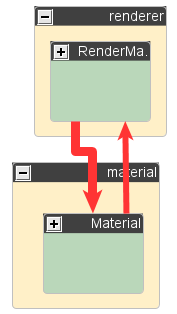
\includegraphics[width=40mm]{figures/dip-violation.png}
\vspace{-15pt}
\caption{A DIP violation}
\label{fig:dip-violation}
\vspace{-60pt}
\end{wrapfigure}

The layer for rendering should be a higher layer than the
layer with materials.
Therefore, the dependency inversion principle requires
the material layer to implement an interface of some sort
in the renderer layer.
However, in the current system the \verb|com.jme3.renderer| package 
depends on the \verb|com.jme3.material| package.
Or more specific: the RenderManager uses the Material class directly.
As can be seen in 
\hyperref[fig:dip-violation]{Figure~\ref*{fig:dip-violation}}.

This means that changes to the Material class will propagate
to the RenderManager and it is not easy to replace the current
implementation of Material.

% extra space to stop wrapping arounf the figure
\vspace{45pt}

\subsection{Acyclic Dependency Principle violation}
\label{sec:adp_violation}
% One example of an Acyclic Dependency Principle violation

The packages \verb|com.jme3.material|, \verb|com.jme3.renderer| and
\verb|com.jme3.scene| together violate the ADP on the package level:

\begin{wrapfigure}{l}{55mm}
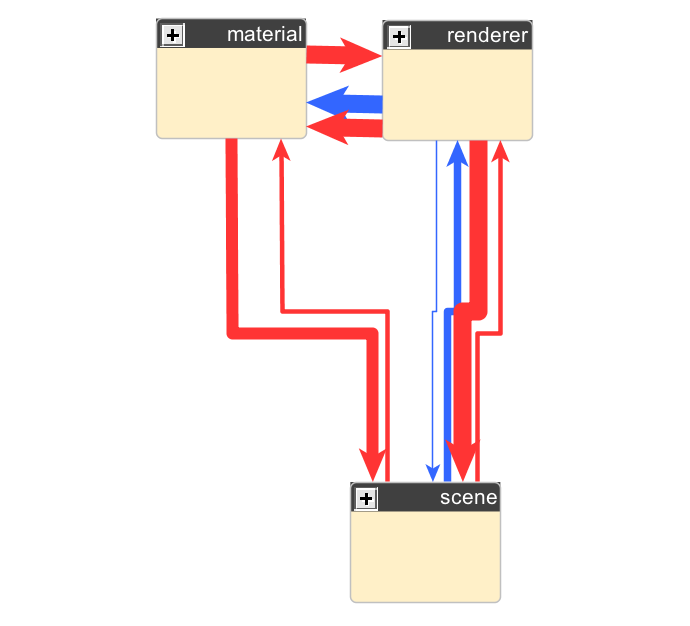
\includegraphics[width=200px, height=200px]{figures/adp-violation.png}
\caption{An acyclic dependency principle violation. Red arrows
  represent method invocations while their thickness represents the
  number of invocations}
\label{fig:adp-violation}
\end{wrapfigure}

They call each other's methods: In one direction (the 3 packages
actually form 2 cycles), \textbf{26} methods contained in classes in
\verb|com.jme3.material| are invoking methods in classes in
\verb|com.jme3.renderer|, \textbf{33} methods in classes in
\verb|com.jme3.renderer| are calling methods contained in classes in
\verb|com.jme3.scene| and \textbf{4} methods contained in classes in
\verb|com.jme3.scene| are calling methods contained in classes in
\verb|com.jme3.material|.

The reason the ADP violation is a problem is that the packages become
tightly coupled, which means that deployment becomes more difficult as
now at least these 3 (and possibly more) packages cannot be
independently deployed.
Modifying the classes within these packages also becomes more
difficult as there is no coherent interface to the subsystems the
packages represent while at the same time the consequences of these
modifications become harder to predict.\\

\subsection{Don't Repeat Yourself violation}
\label{sec:dry_violation}
% One example of a Don't Repeat Yourself violation

The function \verb|distanceSquared(LineSegment)| in the package\\
\verb|com.jme3.math.LineSegment| clearly violates the DRY principle,
as the same code structure is repeated over and over again. As it turns
out, the LineSegment class contains \textbf{24} of such duplicate code
blocks while the cyclomatic complexity of the method is
\textbf{37}. Furthermore, the method is \textbf{284} SLOC long and has
\textbf{197} statements in it. Together these extremely high numbers
indicate that the method is difficult to understand and therefore
difficult to maintain.

% Metrics com.jme3.math.LineSegment.distanceSquared(LineSegment):
% number of duplicate code blocks: 24
% Cyclomatic complexity (branches): 37
% LOC per method: 284
% number of statements: 197
% All caused by the code duplication

The following snippet was taken from Region 1 according to the
accompanying comment, and runs through lines 218-222. The snippet
looks like this:
\begin{code}
  tempS1 = -(negativeDirectionDot * s0 + diffTestDot);
  if (tempS1 < -test.getExtent()) {
    s1 = -test.getExtent();
    squareDistance = s1 * (s1 - (2.0f) * tempS1)
    + s0 * (s0 + (2.0f) * diffThisDot)
    + lengthOfDiff;
\end{code}

The \verb|if|-statement is not closed because line 223 starts an
\verb|else if|-statement, which is a duplicate form of this one
w.r.t. structure.

% The method \verb|com.jme3.math.ColorRGBA.clamp()| performs
% manipulations on the \verb|com.jme3.math.ColorRGBA.{r,g,b,a}|
% fields, but the code is identical in structure for each field.\\
% This is a problem because this code is more difficult to maintain
% than when the functionality is properly factored out.
% Therefore, one possible fix is to rewrite the code to something like:
% \begin{code}
%   private float clampInternal(float val) {
%     if (val < 0) {
%       val = 0;
%     } else if (val > 1) {
%       val = 1;
%     }
%   }
%
%   public void clamp() {
%     this.r = clampInternal(this.r);
%     this.g = clampInternal(this.g);
%     this.b = clampInternal(this.b);
%     this.a = clampInternal(this.a);
%   }
% \end{code}

% \subsection{Other class and package design violations}
% \label{sec:other_violations}
% % This one is optional; If we have the time I recommend we do it - Joey

\newpage
\section{Used tools}
\label{sec:used_tools}

Below is a list of the analysis and refactoring tools we used.
% separated into \emph{static analysis} and \emph{dynamic analysis}.

% \subsection{Static analysis}
% \label{sec:static_analysis}

\begin{enumerate}[i)]
\item \textbf{inCode} is an Eclipse plugin that generates \emph{class
    blueprints} from Java source code.
\item \textbf{Sonar}
	is a tool which entails several code checking tools like PMD and FindBugs. It also checks for metrics like complexity, code duplicates and coupling.
	The findings are easily browsable via the Sonar server.
\item \textbf{Eclipse Metrics} is and eclipse plugin 
	that checks for a collection of metrics.
	It places markers at the source code, but can also
	export its findings to a browsable HTML format.
\end{enumerate}

% \subsection{Dynamic analysis}
% \label{sec:dynamic_analysis}

% \begin{enumerate}[i)]
% \item \textbf{}
% \end{enumerate}

\section{Appendix A: Tables}
The tables listed here contain more detailed information on the
previous chapters.

\begin{table}
  \caption{Vla met pizza}
\begin{tabular}{| c | c |}
  \hline
  \textbf{Feature}                  & \textbf{Important source entities} \\
  \hline
  \hline
  Managing assets                   & AssetManager, ImplHandler, \\
				    & Node, Mesh, Geometry, Spatial \\
  \hline
  Creating applications             & SimpleApplication \\
  \hline
  Managing/configuring applications & AppSettings, JmeSystem, \\
                                    & JmeSystemDelegate, \\
                                    & AbstractAppState, AppStateManager \\
  \hline
  Real time rendering               & RenderManager, Camera,  \\
                                    & ViewPort, RenderQueue \\
  \hline
  Shaders                           & Shader, Uniform, \\
                                    & UniformBindingManager \\
  \hline
  Collision Detection		    & CollisionResults, BoundingVolume\\
  \hline
\end{tabular}

\end{table}

\end{document}
